\begin{figure}
	\centering
	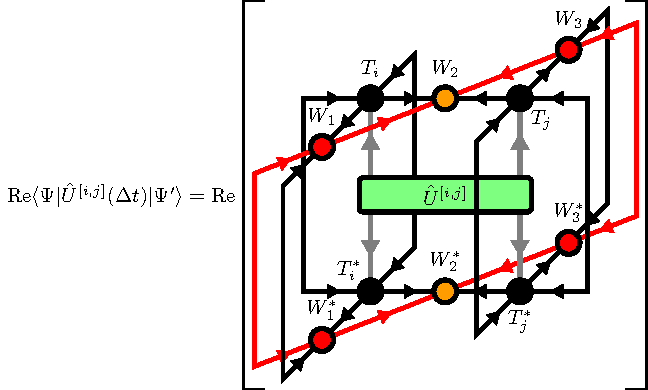
\includegraphics[scale=1]{figures/tikz/disoTPS/tebd_environment/tebd_environment.pdf}
	\caption{(a The five tensor environment of the bond on which the bond operator is to be applied. All arrows are incoming. (b) Definitions of the sub-networks $\mathcal{C}$ and $\mathcal{C}^\prime$ used in equation \eqref{eq:isoDTPS_TEBD_local_update_error}.}
	\label{fig:disoTPS_TEBD_definition_of_environment}
\end{figure}
Let us assume that the orthogonality center is positioned between the two sites on which the bond operator $\hat{U}^{[x, y]}\left(\Delta t\right)$ acts. The five tensors around the orthogonality center then make up a sub-network with only incoming arrows, see figure \figref{fig:disoTPS_TEBD_five_tensor_environment}. We call these five tensors $T_1$, $T_2$, $W_1$, $W_2$ and $W_3$. The local TEBD update can then be formulated as the following problem: Find tensors $T_1^\prime$, $T_2^\prime$, $W_1^\prime$, $W_2^\prime$ and $W_3^\prime$ satisfying the isometry constraints and minimizing the error
\begin{equation}
	\label{eq:isoDTPS_TEBD_local_update_error}
	\varepsilon_\text{trunc} = \left\lVert \hat{U}^{[x,y]}(\Delta t)|\Psi\rangle - |\Psi\rangle\right\rVert = \underset{T_1^\prime, T_2^\prime, W_1^\prime, W_2^\prime, W_3^\prime}{\argmax}\Re\langle\Psi|\hat{U}^{[x,y]}(\Delta t)|\Psi^\prime\rangle.
\end{equation}
Using the isometry condition, the overlap $\langle\Psi|\hat{U}^{[x,y]}(\Delta t)|\Psi^\prime\rangle$ can be comput by contracting the tensor network drawn in figure \figref{fig:disoTPS_TEBD_contraction_definition}. For solving this problem we again use the Evenbly-Vidal algorithm. As we already did in section \ref{sec:YB_move_iterative_local_optimization} for the YB move, we optimize one tensor at a time while keeping all other tensors fixed. This procedure is then repeated, sweeping over all five tensors until convergence is achieved. For more details on this optimization method see appendix \ref{app:riemannian_optimization_of_isometries}. Since the time step $\Delta t$ is chosen to be small, the bond operator is close to identity, $\hat{U}^{[x,y]}(\Delta t)\approx\id$. Thus, a good initialization for the tensors of the updated wavefunction $|\Psi^\prime\rangle$ are simply the tensors of the old wavefunction $|\Psi\rangle$. \par
The computational complexity of applying a local bond operator to a disoTPS with the discussed algorithm scales as $\mathcal{O}(\chi^3D^3d^2) = \mathcal{D^6}$. \todo{Talk about convergence!}